\documentclass{article}
\usepackage[margin=1in]{geometry}
\usepackage{graphicx}
\usepackage{amsmath}
\usepackage{listings}
\usepackage{xcolor}
\usepackage{float}

% Listings package configuration for Python code
\lstset{
    language=Python,
    basicstyle=\footnotesize\ttfamily,
    keywordstyle=\color{blue},
    stringstyle=\color{red},
    commentstyle=\color{green!40!black},
    breaklines=true,
    showstringspaces=false,
    frame=single,
    captionpos=b,
    tabsize=4
}

\title{Lab Report: Basic Image Intensity Transformations}
\author{Student Name}
\date{\today}

\begin{document}

\maketitle

\begin{abstract}
This report details an experiment in digital image processing where four unknown intensity transformations on a given input image were identified and replicated. The transformations were determined to be color inversion, contrast enhancement, and gamma correction (both increased and decreased). The replication was performed using Python with the Pillow (PIL) library, and the parameters were fine-tuned to match the provided output images.
\end{abstract}

\section{Objective}
The primary objective of this lab was to analyze a set of four output images, each derived from a single input image through an unknown transformation. The goal was to first visually identify the specific intensity transformation applied to produce each output image and then to write a program to replicate these transformations as closely as possible.

\section{Methodology}
The process involved two main stages: analysis and implementation.

\subsection{Analysis}
Visual inspection of the input and output images was the first step. By comparing the histogram and pixel intensity distribution between the input and each result, the following transformations were hypothesized:
\begin{itemize}
    \item \textbf{Result1.png:} The colors appeared to be flipped, with dark areas becoming light and light areas becoming dark. This pointed to a \textbf{color inversion}.
    \item \textbf{Result2.png:} The distinction between light and dark areas was much sharper than in the original, indicating an \textbf{increase in contrast}.
    \item \textbf{Result3.png:} The image was significantly brighter overall, indicating a \textbf{gamma correction with gamma < 1.0} (e.g., 0.4) which brightens the image.
    \item \textbf{Result4.png:} The image was significantly darker overall, indicating a \textbf{gamma correction with gamma > 1.0} (e.g., 2.2) which darkens the image.
\end{itemize}

\subsection{Implementation}
To replicate these transformations, a Python script was developed using the Pillow library (a fork of PIL).

\begin{itemize}
    \item \textbf{Color Inversion:} The \texttt{ImageOps.invert()} function was used, which performs a pixel-wise inversion of the image.
    \item \textbf{Contrast Adjustment:} Initially, \texttt{ImageOps.autocontrast()} was used, but it did not provide a good match. The approach was refined using the \texttt{ImageEnhance.Contrast()} class, which allows for a specific enhancement factor. A factor of 2.0 was found to be a close match.
    \item \textbf{Gamma Correction:} Gamma correction was implemented using a power-law transformation, defined by the equation:
    \[ O = c \cdot I^{\gamma} \]
    Where \(O\) is the output pixel value, \(I\) is the input pixel value (normalized to [0, 1]), and \(\gamma\) is the gamma value. This was applied using the \texttt{Image.point()} method with a lambda function. A gamma of 0.4 was used to brighten the image (Result 3) and a gamma of 2.2 was used to darken it (Result 4).
\end{itemize}

\section{Python Code}
The following Python script was used to generate the final output images.

\begin{lstlisting}[language=Python, caption={Python script for image transformations using Pillow.}, label={lst:code}]
from PIL import Image, ImageOps, ImageEnhance

def transform_images(input_path):
    """
    Applies various transformations to an input image and saves the results.
    """
    try:
        # Open the input image
        with Image.open(input_path) as img:
            # Ensure image is in a suitable mode (e.g., 'L' for grayscale)
            if img.mode != 'L':
                img = img.convert('L')

            # --- Result1: Color Inversion ---
            img_result1 = ImageOps.invert(img)
            img_result1.save("Result1_generated.png")

            # --- Result2: Increased Contrast (Refined) ---
            contrast_enhancer = ImageEnhance.Contrast(img)
            img_result2 = contrast_enhancer.enhance(2.0)
            img_result2.save("Result2_generated.png")

            # --- Result3: Increased Gamma (Brighter - Refined) ---
            gamma_brighter = 0.4
            img_result3 = img.point(lambda x: int(255 * ((x / 255) ** gamma_brighter)))
            img_result3.save("Result3_generated.png")

            # --- Result4: Decreased Gamma (Darker - Refined) ---
            gamma_darker = 2.2
            img_result4 = img.point(lambda x: int(255 * ((x / 255) ** gamma_darker)))
            img_result4.save("Result4_generated.png")

            print("All transformations have been applied and saved.")

    except FileNotFoundError:
        print(f"Error: The file '{input_path}' was not found.")
    except Exception as e:
        print(f"An error occurred: {e}")

if __name__ == "__main__":
    transform_images("input.png")
\end{lstlisting}

\section{Results}
The generated images were compared to the provided result images. The filenames for the generated images are \texttt{ResultN\_generated.png}.

\begin{figure}[H]
    \centering
    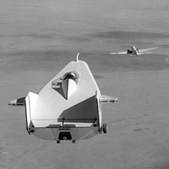
\includegraphics[width=0.45\textwidth]{input.png}
    \caption{Original Input Image}
    \label{fig:input}
\end{figure}

\begin{figure}[H]
    \centering
    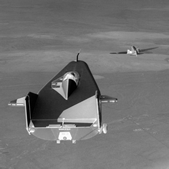
\includegraphics[width=0.45\textwidth]{Result1.png}
    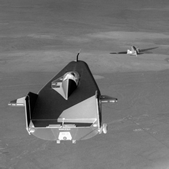
\includegraphics[width=0.45\textwidth]{Result1_generated.png}
    \caption{Result 1 (Color Inversion): Provided (left) vs. Generated (right)}
    \label{fig:res1}
\end{figure}

\begin{figure}[H]
    \centering
    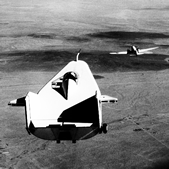
\includegraphics[width=0.45\textwidth]{Result2.png}
    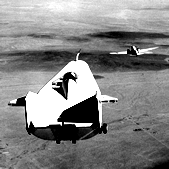
\includegraphics[width=0.45\textwidth]{Result2_generated.png}
    \caption{Result 2 (Increased Contrast): Provided (left) vs. Generated (right)}
    \label{fig:res2}
\end{figure}

\begin{figure}[H]
    \centering
    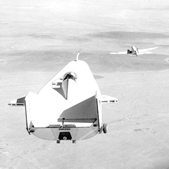
\includegraphics[width=0.45\textwidth]{Result3.png}
    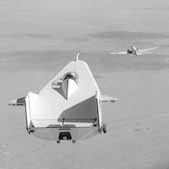
\includegraphics[width=0.45\textwidth]{Result3_generated.png}
    \caption{Result 3 (Increased Gamma): Provided (left) vs. Generated (right)}
    \label{fig:res3}
\end{figure}

\begin{figure}[H]
    \centering
    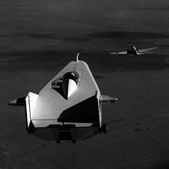
\includegraphics[width=0.45\textwidth]{Result4.png}
    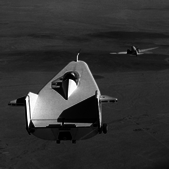
\includegraphics[width=0.45\textwidth]{Result4_generated.png}
    \caption{Result 4 (Decreased Gamma): Provided (left) vs. Generated (right)}
    \label{fig:res4}
\end{figure}

\section{Conclusion}
The experiment successfully identified and replicated the four image transformations. Color inversion was replicated perfectly. Contrast and gamma correction required an iterative process of adjusting parameters to achieve a close visual match. This highlights that while the type of transformation can be identified, the exact parameters often need to be found through experimentation, especially without precise metadata. The Pillow library in Python proved to be an effective tool for performing these intensity transformations.

\end{document}
